\documentclass[dvipdfmx]{jsarticle}
\usepackage[dvipdfmx]{graphicx}
\usepackage{amsmath}
\usepackage{amssymb}
\usepackage{amsfonts}
\usepackage{mathrsfs}
\usepackage{bm}
\usepackage{bbm}
\usepackage{braket}
\usepackage[english]{babel}
\usepackage{here}
\usepackage{comment}
\usepackage{longtable}
\usepackage{cancel}
\allowdisplaybreaks[4]
\usepackage{tikz}
\usepackage{simpler-wick}
%\begin{comment}
\usetikzlibrary{positioning}
  \makeatletter
%  \renewcommand{\theequation}{\arabic{chapter}-\arabic{section}-\arabic{equation}}
  \renewcommand{\theequation}{\arabic{section}.\arabic{subsection}.\arabic{equation}}
  \@addtoreset{equation}{section}
  \@addtoreset{equation}{subsection}
%\end{comment}
  \makeatother
  \usepackage[left=25truemm,top=20truemm,bottom=20truemm,right=25truemm]{geometry}
\usepackage[dvipdfmx]{hyperref}
\usepackage{pxjahyper}
\usepackage{url}
\title{Lie代数から学ぶ量子力学と場の量子論}
\author{東京大学大学院 Kavli IPMU 立川研究室 \hspace{15pt}Shin TOITA\thanks{e-mail: shintaro.toita@ipmu.jp}}

\begin{document}
\newgeometry{left=25truemm,top=-5truemm,bottom=20truemm,right=25truemm}
\maketitle
\vspace{-4zh}

\tableofcontents
ToDo:
\\grad, div, rot
\\scalarの変換性とvectorの変換性
\\無限に深い井戸型ポテンシャル、波動関数の境界条件
\\電磁場のgauge対称性と波動関数の位相、特異系のLagrangian
\\Planckの光量子仮説 
\\簡単なベクトル解析、完全反対性テンソル
\\配位空間と相空間、symplectic幾何、正準変換
\\電磁場中の古典荷電粒子、電磁場中の一般化運動量
\\昇降演算子(n粒子系と1粒子系の第n励起の区別)
\\固有関数の完全性(離散変数、連続変数)
\\束縛状態の基礎(連続性、境界条件、規格化可能性、tunneling効果、
\\Heisenbergの運動方程式、Ehrenfestの定理)、
\\規格化(離散変数、連続変数)
\\非エルミートな演算子の固有状態(Coherent state、Whittaker state)、位相演算子
\\簡単な散乱問題、ポテンシャル共鳴
\newgeometry{left=25truemm,top=25truemm,bottom=20truemm,right=25truemm}
\section{質点の解析力学の基礎}

\subsection{Newton力学}

皆さんが良く知っているNewtonの運動方程式
\begin{align}
  \bm{F} = m\ddot{\bm{x}}
\end{align}
は解析力学に比べて最も一般的な運動方程式の形で、
例えば摩擦力が働くなどenergy散逸のある系や
外部から力を受けている系などを何の困難もなく表すことが出来る。

例えば1次元調和振動子の場合を考えると
\begin{align}
  F = -k x
\end{align}
であるので、Newton運動方程式は
\begin{align}
  m\ddot{x} = - k x
\end{align}
となる。

ただし、この方程式はvectorで記述されているため、
例えば極座標のような直交座標系以外の座標を用いると
形が著しく複雑になるという欠点も持っている。
これに対し、例えばenergyのようなscalar量は
座標変換の下でより自然に変換するため、
様々な力学法則をscalarを用いて表したいというのは自然な要求である。
以下で議論するLagrange力学やHamilton力学はそのような
記述を与える枠組みの例である。

\subsection{Lagrange力学}

多くの力学系において、
位置$\bm{x}$にある粒子に働く力は
位置の関数$\bm{F}(\bm{x})$と書ける。
この関数$\bm{F}$のように空間の各点$\bm{x}$に対し
あるvector $\bm{F}(\bm{x})$を与えるものを
vector値関数、あるいはvector場という。

物体に働く力$\bm{F}$が保存力である
\begin{align}
  \mathrm{rot} \bm{F}
  := 
  \nabla \times \bm{F}
  = 0
\end{align}
場合にはscalar potential $\phi(\bm{x})$
が存在して
\begin{align}
  \bm{F} = -\nabla \phi
\end{align}
と書けることは、力学で最初に習う事の一つだろう。

我々の主たる興味は空間が3次元である場合にあるが、
この場合にはより一般的な結果が知られている:
Helmholtzの分解定理は任意の
3次元vector場$\bm{F}(\bm{x})$に対し
vector potential $\bm{A}(\bm{x})$と
scalar potential $\phi(\bm{x})$の組であって
\begin{align}
  \bm{F}(\bm{x}) = \nabla \times \bm{A} - \nabla \phi
\end{align}
なるものが存在する事を主張する。
つまり、物体に働く力が場である
(顕わに時間依存したりすることなく、位置のみの関数として書けている)
限りにおいて、
必ずvector potential及びscalar potentialを用いて書けるのである。

これを踏まえ、
まずは物体に働く力がscalar potentialを用いて書ける場合に
話を限ろう。
3次元空間に記述したい質点が$n$個あるとすれば、
これらの質点の状態は
一般化座標$q_i$$(i=1,2,\dots,3n)$を用いて記述できる。
これらをまとめて$\{q\} := \{q_i| i=1,2,\dots,3n\}$と書く。
ここで我々の世界がNewtonの運動方程式のように
決定論的な力学法則に支配されていると信じると、
これらの力学変数$q_i$は各時刻で完全に決定されているはずなので、
時間の関数$q_i(t)$として与えられている。
よって時間微分が定義でき、
$\dot{q}(t) := \dfrac{dq(t)}{dt}$
と書く。

Newton以来の経験的事実として、
我々の世界の力学法則はこれらの座標の2階までの時間微分で記述できるため、
kinetic energy $T$と
potential energy $V$
が
$\{q\}, \{\dot{q}\}$の関数として表される事は事実として受け入れよう。
このとき、Lagrangian $L(\{q\}, \{\dot{q}\})$を
$6n$変数関数として
\begin{align}
  L := T - V
\end{align}
で定義する。
個々の力学変数$q_i(t)$は時間の関数であるので、
$6n$変数関数
$L(\{q\}, \{\dot{q}\})$との合成関数
$L(t) := L(\{q(t)\}, \{\dot{q}(t)\})$は時間の$1$変数関数であり、
時刻$t_i$から時刻$t_f$までの定積分が定義できる:
\begin{align}
  S := \int_{t_i}^{t_f}dt\ L(\{q\}(t), \{\dot{q}\}(t))
\end{align}
この$S$をaction(作用)と言い、$I$と書くこともある。

最小作用の原理は、個々の力学変数の時間依存性は
このactionが停留するような関数形で与えられる事を主張する。
つまり、$q_i(t)$を時間の関数と見做したときの関数形を
\begin{align}
  q_i(t) &\mapsto (q_i+\delta q_i)(t) := q_i(t) + \delta q_i(t)
  \\
  | q_i(t) | & \gg | \delta q_i(t) |
  \qquad (\forall t)
\end{align}
のように微小に変化させたとき、
どんな関数$\delta q_i(t)$に対しても
actionの変分
\begin{align}
  \delta S &:= \int dt\ L(\{ q_i(t) + \delta q_i(t) \},
  \{ \dot{q}_i(t) + \delta \dot{q_i}(t) \} )
\notag\\&\simeq
  \int dt\ \sum_i
  \bigg\{
    \delta q_i(t)
    \dfrac{\partial}{\partial q_i}
    L(\{ q(t) \},
    \{ \dot{q}(t) \} )
%  \notag\\&\qquad
+
    \delta \dot{q_i}(t)
    \dfrac{\partial}{\partial \dot{q_i}}
    L(\{ q(t) \},
    \{ \dot{q}(t) \} )
  \bigg\}
\notag\\&\simeq
\int dt\ \sum_i
\delta q_i(t)
\bigg\{
  \dfrac{\partial}{\partial q_i}
  L(\{ q(t) \},
  \{ \dot{q}(t) \} )
%  \notag\\&\qquad
-
  \dfrac{d}{dt}
  \dfrac{\partial}{\partial \dot{q_i}}
  L(\{ q(t) \},
  \{ \dot{q}(t) \} )
\bigg\}
%  \qquad (\ \forall\ \delta q_i(t), i\ )
\end{align}
(ここで、部分積分による表面項が現れない事
$[\cdots]_{t=t_i}^{t_f}=0$
を仮定した)
が消えること
\begin{align}
  \delta S &= 0
  \qquad (\forall\ \delta q_i(t), i)
\\\Leftrightarrow\qquad
  0 &= 
  \dfrac{d}{dt}\dfrac{\partial L}{\partial \dot{q_i} }
  - \dfrac{\partial L}{\partial q_i }
  \qquad (\ \forall i\ )
\label{Euler-Lagrange for point masses}
\end{align}
を要求すると、得られた微分方程式の解が
物理的に実現される物体の軌跡${q(t)}$
を与えるというのである。
(\ref{Euler-Lagrange for point masses})
をEuler-Lagrange方程式と言い、
scalar量$L$によって力学法則を与えたという点で
確かに目標を達成している。
実際、$\{q\}$から新しい変数$\{ q'\}$への座標変換
$q_i = q_i(\{q'\})$
のもとでEuler-Lagrange方程式が形を変えないことが示される。

\subsubsection{調和振動子の例}

$n$次元調和振動子の場合Lagrangianは
\begin{align}
  L = \sum_{j=1}^n
  \bigg(
    \dfrac{m}{2}\dot{q_j}^2
  -
    \dfrac{m\omega^2}{2} q_j
  \bigg)
\end{align}
であるので、Euler-Lagrange方程式は
\begin{align}
  0 &= 
  \dfrac{d}{dt}\dfrac{\partial L}{\partial \dot{q_i} }
  - \dfrac{\partial L}{\partial q_i }
\notag\\&=
  \dfrac{d}{dt}
  \bigg(
    m\dot{q_i}
  \bigg)
  - 
  \bigg(
  -
    m\omega^2 q_i
  \bigg)
\notag\\&=
    m\ddot{q_i}
  +
    m\omega^2 q_i
\end{align}
となり、確かにNewtonの運動方程式を再現する。

\subsection{Hamilton力学}

一般にEuler-Lagrange方程式は各変数$q_i$の
高階の微分を含む、複雑な方程式系となる。
変数を増やす代わりに、
低次の微分で書ける方程式系を見付けたいと思うのも自然な発想である。
Lagrangian $L(\{q\},\{\dot{q}\})$に
新しい変数$\{p\}$を導入する代わりに
$\dot{q}_i$を消去し、
Euler-Lagrange方程式と等価な微分方程式系を得ることを考えよう。

一般化運動量を
\begin{align}
  p_i := \dfrac{\partial L}{\partial \dot{q_i}}
\label{generalized momentum}
\end{align}
で定義する。
一般に$\det \dfrac{\partial^2 L}{\partial \dot{q_i} \partial \dot{q_j} } \neq 0 $
であれば
$p$の定義式を$\dot{q_i}$について
\begin{align}
  \dot{q_i} = \dot{q_i}(\{q\},\{p\},t)
\end{align}
のように解く事が出来、
\footnote{
  このような逆解きが出来ない力学系を
  特異Lagrange系と呼ぶ。
  gauge理論などは場の量子論における特異系の例である。
}
従って$\dot{q_i}$を方程式系から消去できる。
Euler-Lagrange方程式は
\begin{align}
  \begin{cases}
    \dot{p_i} = \dfrac{\partial L}{\partial q_i}
\\    \\
      p_i = \dfrac{\partial L}{\partial \dot{q_i}}   
  \end{cases}
%\quad
%&\Leftrightarrow
%\quad
\label{Euler-Lagrange with p}
\end{align}
となるが、
Lagrangianそのものから$\{\dot{q}\}$を消去し
$\{q\},\{p\}$の$6n$変数関数として書き直すと
(\ref{generalized momentum})の右辺を表現する方法がなくなってしまう。
そこで別のアプローチを考えよう。

我々が欲しいのは新しい変数で表されたLagrangianそのものではなく、
Lagrangianを古い変数で微分して得られる方程式系である。
そこで、新しい変数$\{q\},\{p\}$で微分すると
Lagrangianを古い変数$\{q\}, \{\dot{q}\}$
で微分したときと等価の式を与えるような、
新しい関数$H(\{q\},\{p\})$を構成することを考える。

Legendre変換
\begin{align}
  H(\{q\},\{p\})
  :=
  \bigg[
    \sum_i 
      \dot{q_i} p_i
  - L(\{q\}, \{\dot{q}\})
  \bigg]_{\dot{q} = \dot{q}(\{q\},\{p\},t)}
\end{align}
はそのような構成の例である。
右辺には$9n$個の変数$\{q\},\{\dot{q}\},\{p\}$が表れているが、
$\dot{q}$が消去され
$\{q\},\{p\}$の$6n$変数関数として表されていることに注意しよう。
関数$H$をHamiltonianというが、
その著しい性質は$\dot{q}$を消去する直前の表式が
$\dot{q}$に依っていないこと
\begin{align}
  \dfrac{\partial}{\partial \dot{q_i}}
  \bigg[
    \sum_j
      \dot{q_j} p_j
  - L(\{q\}, \{\dot{q}\})
  \bigg]
  &=
  \bigg[
    \sum_j\bigg(
      \delta_{ij} p_j
    \bigg)
  - \dfrac{\partial L}{\partial \dot{q_i}}
  \bigg]
\notag\\&=
  \bigg[
    p_i
    - \dfrac{\partial L}{\partial \dot{q_i}}
  \bigg]
\notag\\
  &=0
\end{align}
である。
ただし、偏微分は$\{q\},\{\dot{q}\},\{p\}$の全てを独立な変数と見做して
行っていることに注意せよ。

Hamiltonianの$\{q\},\{p\}$による微分は、
$q(t)$がEuler-Lagrange方程式の解であるとすると
\begin{align}
  \dfrac{\partial H}{\partial q_i} 
  &= 
  \dfrac{\partial}{\partial q_i} 
  \bigg[
    \sum_j p_j
     \dot{q_j}
     - L(\{q\}, \{\dot{q}\})
  \bigg]_{\dot{q} = \dot{q}(\{q\},\{p\},t)}
\notag\\  &= 
  \sum_j    p_j
   \dfrac{\partial \dot{q_j} (\{q\},\{p\},t) }{\partial q_i }
   - \dfrac{\partial L(\{q\}, \{\dot{q}(\{q\},\{p\},t)\} ) }{
     \partial q_i
   }
\notag\\  &= 
   \sum_j    p_j
    \dfrac{\partial \dot{q_j} }{\partial q_i}
    - \Bigg[
      \dfrac{\partial L(\{q\}, \{\dot{q}\} ) }{
        \partial q_i
      }\bigg|_{\dot{q} = \dot{q}(\{q\},\{p\},t)}
      +
      \sum_j
      \dfrac{\partial \dot{q_j}}{\partial q_i}
      \dfrac{\partial L(\{q\}, \{\dot{q}\} ) }{
        \partial \dot{q_j}
      }\bigg|_{\dot{q} = \dot{q}(\{q\},\{p\},t)}
    \Bigg]
\notag\\  &= 
    \sum_j    p_j
     \dfrac{\partial \dot{q_j} }{\partial q_i}
     - \Bigg[
       \dfrac{\partial L(\{q\}, \{\dot{q}\} ) }{
         \partial q_i
       }\bigg|_{\dot{q} = \dot{q}(\{q\},\{p\},t)}
       +
       \sum_j
       \dfrac{\partial \dot{q_j}}{\partial q_i}
       p_j
     \Bigg]
\notag\\  &= 
      - 
        \dfrac{\partial L(\{q\}, \{\dot{q}\} ) }{
          \partial q_i
        }\bigg|_{\dot{q} = \dot{q}(\{q\},\{p\},t)}
\notag\\  &= 
      - 
      \dfrac{ d }{ dt }
      \dfrac{\partial L}{
        \partial \dot{q_i}
      }
    \qquad\because\text{Euler-Lagrange方程式}  
\notag\\  &= 
    - 
    \dot{p_i}
\label{Hamilton's eom1}
\\
  \dfrac{\partial H}{\partial p_i} 
  &= 
  \dfrac{\partial }{\partial p_i} 
  \bigg[
    \sum_j
      \dot{q_j} p_j
  - L(\{q\}, \{\dot{q}\})
  \bigg]_{\dot{q} = \dot{q}(\{q\},\{p\},t)}
\notag\\  &= 
  \sum_j
  \bigg[
    \dfrac{\partial \dot{q_j}(\{q\},\{p\},t)}{
      \partial p_i
    } p_j
  +
  \dot{q_j}(\{q\},\{p\},t) \delta_{ij}
  \bigg]
- \dfrac{\partial L(\{q\}, \{\dot{q}\}) }{
  \partial p_i
}
\bigg|_{\dot{q} = \dot{q}(\{q\},\{p\},t)}
\notag\\  &= 
  \sum_j
    \dfrac{\partial \dot{q_j}}{
      \partial p_i
    } p_j
  +
  \dot{q_i}
  - \sum_j
  \dfrac{\partial \dot{q_j} }{
    \partial p_i
  }
  \dfrac{\partial L(\{q\}, \{\dot{q}\}) }{
    \partial \dot{q_j}
  }
  \bigg|_{\dot{q} = \dot{q}(\{q\},\{p\},t)}
\notag\\  &= 
  \sum_j
    \dfrac{\partial \dot{q_j}}{
      \partial p_i
    } p_j
  +
  \dot{q_i}
  - \sum_j
  \dfrac{\partial \dot{q_j} }{
    \partial p_i
  }
    p_j
\notag\\  &= 
    \dot{q_i}
\label{Hamilton's eom2}
\end{align}
のようにLagrangianを一切使わずに表せ、
逆にHamiltonianを再びLegendre変換したものに
(\ref{Hamilton's eom1}),(\ref{Hamilton's eom2})
の解$\{q(t)\},\{p(t)\}$を代入すると
$\{q\},\{p\}$で書いたEuler-Lagrange方程式
(\ref{Euler-Lagrange with p})
を再現する。
すなわち両者は微分方程式系として等価であり、
(\ref{Hamilton's eom1}), 
(\ref{Hamilton's eom2})を
Hamiltonの正準方程式という。

Hamiltonの方程式はscalar関数$H$から得られ、
1階の時間微分のみを含むので、
望む方程式系が得られたことになる。

\subsubsection{調和振動子の例}

$n$次元調和振動子の一般化運動量は
\begin{align}
  p_i &= \dfrac{\partial L}{\partial \dot{q_i}}
=
  m \dot{q_i}
\end{align}
と通常の運動量の定義に一致するので、
Hamiltonianは
\begin{align}
  H &= \bigg[
    \sum_i p_i \dot{q_i}
    - L
    \bigg]_{ \dot{q_i} = \frac{p_i}{m} }
\notag\\&=
    \sum_i p_i \frac{p_i}{m}
    - 
      \sum_i \bigg(
      \dfrac{p_i^2}{2m}
    -
      \dfrac{ m \omega^2 }{2}
      q_i^2
    \bigg)
\notag\\&=
    \sum_i \bigg(
      \dfrac{p_i^2}{2m}
    +
      \dfrac{ m \omega^2 }{2}
      q_i^2
    \bigg)
\end{align}
となる。
正準方程式は
\begin{align}
  \begin{cases}
    \dot{q_i} &= \dfrac{\partial H}{\partial p_i}
    = \dfrac{p_i}{m}
  \\\\
    \dot{p_i} &= - \dfrac{\partial H}{\partial q_i}
    = - m \omega^2 q_i  
  \end{cases}
\quad
\Leftrightarrow
\quad
  \ddot{q_i} &= \dfrac{\dot{p_i}}{m}
  = \dfrac{- m \omega^2 q_i}{m} 
  = - \omega^2 q_i
\end{align}
となって、やはりNewtonの方程式を再現する。

\subsubsection{Poisson括弧}

Hamiltonの正準方程式
\begin{align}
   \begin{cases}
      \dot{q_i} &= \dfrac{\partial H}{\partial p_i}
    \\\\
      \dot{p_i} &= - \dfrac{\partial H}{\partial q_i}
    \end{cases}
\label{Hamilton's eom}
\end{align}
は$\{q\},\{p\}$のいずれについても
時間の1階微分しか含まない点で美しいが、
$\{q\},\{p\}$に対して右辺の符号が異なるという非対称性がある。
より抽象的な演算を導入することで、この非対称性を取り除こう。

2つの量$A,B$のPoisson括弧を
\begin{align}
    \{A, B\}_{ \mathrm{P} }
    := \sum_i \bigg(
        \dfrac{ \partial A }{ \partial q_i }
        \dfrac{ \partial B }{ \partial p_i }
    -
        \dfrac{ \partial B }{ \partial q_i }
        \dfrac{ \partial A }{ \partial q_i }
    \bigg)
\end{align}
で定義すると、
正準方程式(\ref{Hamilton's eom})は
\begin{align}
    \begin{cases}
        \dot{q_i} = \{q_i, H\}_{ \mathrm{P} }
      \\
        \dot{p_i} = \{p_i, H\}_{ \mathrm{P} }
      \end{cases}
\quad
\therefore
\quad
    \dot{r} &= \{r, H\}_{ \mathrm{P} }
\qquad
    ( r = q_i, p_j \quad\forall i, j )
\end{align}
と書ける。
より一般に、任意の関数
$F( \{q\},\{p\} , t )$
の時間発展が
\begin{align}
    \dfrac{ d F }{ dt } &= \dfrac{ \partial F }{ \partial t } + \{F, H\}_{ \mathrm{P} } 
\end{align}
と一つの式にまとまってしまう。
あらゆる量の時間発展を求める過程が、
Poisson括弧の計算という一つの操作に統一されたのである。

なお、正準変数同士のPoisson括弧は
\begin{align}
   \{q_i, p_j\}_{ \mathrm{P} }
   = \delta_{ij}
,\qquad
   \{p_i, q_j\}_{ \mathrm{P} }
   = - \delta_{ij}
\end{align}
のようになる。

\newpage
\section{量子力学の基礎}

量子力学に特徴的な事は、
物理量が単なる数ではなくHilbert空間に作用する
非可換なoperator(演算子、作用素)となる事である。
観測可能な量はHermitian operatorとなるので、
我々はoperatorとして専らlinearな
Hermitianないしunitary operatorを扱う。

\subsection{正準量子化}

\subsubsection{Hilbert空間とOperator}

量子力学に現れるoperator $O$とは、
写像$O: \mathcal{H} \to \mathcal{H}$
すなわち
ある複素vector space $\mathcal{H}$の
元$\ket{\psi}$に作用して
再びvector space の元
$O\ket{\psi} \in \mathcal{H}$
を与えるものである。

あるoperator $O$が$\mathcal{H}$にlinearに作用している、
あるいはlinearである、とは
\begin{align}
    \text{ For }
        \forall \ket{\psi_1}, \ket{\psi_2}
        \in \mathcal{H}
    \text{ and }
        \forall a,b\in \mathbb{C}
    ,\qquad
        O\Big(
            a \ket{\psi_1}
            +
            b \ket{\psi_2}    
        \Big)
    =
        a O \ket{\psi_1}
        +
        b O \ket{\psi_2}    
\end{align}
であることを言う。
例えば時間反転操作に対応するoperator $T$は
anti-unitary (anti-linearかつunitary)
\begin{align}
    \text{ For }
        \forall \ket{\psi_1}, \ket{\psi_2}
        \in \mathcal{H}
    \text{ and }
        \forall a,b\in \mathbb{C}
    ,\qquad
        T\Big(
            a \ket{\psi_1}
            +
            b \ket{\psi_2}    
        \Big)
    =
        a^* T \ket{\psi_1}
        +
        b^* T \ket{\psi_2}    
\end{align}
なoperatorの重要な例であるが、
以下では専らlinearなものに話を限る。

量子力学では物理量はoperatorで表され、
解析力学で基本的な力学自由度であった
$\{q\},\{p\}$
さえもoperatorとなっている。
我々は任意の観測量の時間発展が決定論的な
物理法則によって記述されることを仮定するが、
一方で直接観測される量はもちろん実数であるので、
まずはこれらの観測量を
$\{\hat{q}\},\{\hat{p}\}$
のようなoperatorと関係付ける方法を考えなければならない。
以下ではこの方法を
Hilbert空間と呼ばれるvector spaceを用いて与えよう。

vector space $\mathcal{H}$が
内積$\eta$を持つとは、
$
\forall \ket{\psi_1}, \ket{\psi_2}
\in \mathcal{H}
$
に対し複素数
$ \braket{ \psi_1 | \psi_2 }
:= \eta(\ket{\psi_1}, \ket{\psi_2})
\in \mathbb{C} $
を与える写像
$\eta: 
\mathcal{H}\times \mathcal{H}
\to \mathbb{C}$
であって、
\begin{align}
    \braket{ \psi | \phi } &= \braket{ \phi | \psi }^*
&\text{(共役対称性)}
\\
            \bra{\phi}\Big(
            a \ket{\psi_1}
        +
            b \ket{\psi_2}
        \Big)
    &=
        a \braket{\phi|\psi_1}
    +
        b \braket{\phi|\psi_2}
    \qquad
    \text{ for } \forall
    a,b\in \mathbb{C}
&\text{(線形性)}
\\
    \braket{ \psi | \psi } \ge 0
    ,\quad&\text{and}\quad
    \braket{ \phi | \phi } = 0
    \Leftrightarrow
    \ket{\phi}=0
&\text{(正定値性)}
\end{align}
を満たすものがあることを言う。
Hilbert空間とは内積空間であって完備な
(直感的には、極限が十分に存在する)
ものを言う。
物理学において時間発展は微分方程式で与えられるので、
微分を定義するために
極限が存在する必要があるのである。

量子力学において決定論的な時間発展方程式に従う力学自由度は
Hilbert空間の元である。
このHilbert空間を状態空間と言い、
その元を状態vectorと呼ぶ。
個々の状態vectorの
時間発展はSchr\"odinger方程式
\begin{align}
    i\hbar \dfrac{d}{dt}
        \ket{\psi(t)}
    &=
    \hat{H} \ket{\psi(t)}
\end{align}
によって与えられる。
ここで$\hbar$は換算Planck定数またはDirac定数と呼ばれ、
Planck定数$h$により
\begin{align}
    \hbar := \dfrac{h}{2\pi}
\end{align}
と定義される。
また、
$\hat{H}$は以下で定義する
Hamiltonian operatorである。

\subsubsection{正準交換関係(CCR: Canonical Commutation Relation)}

二つのoperator $\hat{A}, \hat{B}$の間の交換関係を
\begin{align}
    [\hat{A}, \hat{B}] := \hat{A} \hat{B} - \hat{B} \hat{A}
\end{align}
で定義し、$[\hat{A}, \hat{B}] = 0$であるとき
$\hat{A}, \hat{B}$は可換であるという。
全く同様に反交換を
\begin{align}
    \{\hat{A}, \hat{B}\} := \hat{A} \hat{B} + \hat{B} \hat{A}
\end{align}
で定義しておく。
量子力学を考えるまで、
あらゆる量は可換であった。
このように全ての量が可換である力学系を
古典力学系と言い、そこに現れる可換な数を$c$-数という。

任意の関数$F(a)$について、
演算子$\hat{x}$の関数$F(\hat{x})$を
($a=0$周りの)Taylor展開により
\begin{align}
    F(\hat{x}) := \sum_{n=0}^\infty
        \dfrac{1}{n!}
        \dfrac{d^nF(a)}{da^n}\bigg|_{a=0}
        \hat{x}^n
\label{function of operator}
\end{align}
と定義する。
ある古典力学系のHamiltonian $H(\{q\},\{p\})$
が知られているとき、
その正準力学変数$\{q\},\{p\}$を
正準交換関係:
\begin{align}
    [ \hat{q}_i , \hat{p}_j ] = i\hbar \delta_{ij}
\end{align}
を満たすoperatorの組
$ \{\hat{q}\} , \{\hat{p}\} $
で置き換える手続きを正準量子化と呼び、
\begin{align}
    \hat{H}
    &:=
    H(\{\hat{q}\} , \{\hat{p}\})
\end{align}
を得られた量子力学系の
Hamiltonian operator
という。

厳密にはこれだけでは古典的Hamiltonian $H$が
例えば$qp$のような項を持っていたとき、それを
$\hat{p}\hat{q}$で置き換えるのか
$\hat{q}\hat{p} = \hat{p}\hat{q} + i\hbar$で置き換えるのか
といった問題は残る。
これを演算子順序の問題といい、
Hamiltonian operatorのHermiticityや
量子系の持つべき大域的対称性などから
一定の解答を与えることは出来るものの、
異なる演算子順序は物理的に異なる量子系を与えるため
一般に与えられた古典系に対して量子系を一意に定めることは出来ない。
ただし特定の文脈で自然な演算子順序は存在し、
このことは経路積分を扱う際により詳しく議論する。

\subsubsection{ObservablesとHermitian conjugate}

任意のvector $\ket{\psi} \in \mathcal{H}$の
Hermitian conjugate $\ket{\psi}^\dagger$を
内積を使って
\begin{align}
    \ket{\psi}^\dagger
    :=
    \eta(\ket{\psi},\ )
\end{align}
により定め、$\bra{\psi}$とも書く。
元の空間の任意の元
$\ket{\phi} \in \mathcal{H}$
との内積が
\begin{align}
    \ket{\psi}^\dagger \ket{\phi}
    :=
    \braket{\psi|\phi}
    = \eta(\ket{\psi}, \ket{\phi})
    \in \mathbb{C}
\end{align}
のように複素数を与えるため、
内積の線形性から
$\bra{\psi}$は$\mathcal{H}$上の
線形汎関数と見做すことが出来、
$\bra{\psi}$のなす集合$\mathcal{H}^*$は
$\mathcal{H}$の(位相的あるいは線形)双対空間となる。

この定義の下でoperator $\hat{O}$の
Hermitian conjugate $\hat{O}^\dagger$も、
任意のvector $\ket{\psi}, \ket{\phi}$に対して
\begin{align}
    \bra{\psi}
    \hat{O}^\dagger
    \ket{\phi}
    =
    \ket{\psi}^\dagger
    \hat{O}^\dagger
    \ket{\phi}
    &:=
    \Big( \hat{O} \ket{\psi} \Big)^\dagger
    \ket{\phi}
    =
    \Big[
        \bra{\phi} \Big( \hat{O} \ket{\psi} \Big)
    \Big]^*
\end{align}
となるoperatorと定めることが出来る。

あるoperator $\hat{O}$がHermitianであるとは、
$\hat{O}$が
\begin{align}
    \hat{O} = \hat{O}^\dagger
\end{align}
を満たすことを言う。
量子力学におけるObservable(可換測量)は、
Hermitian operator で表される。

\subsubsection{固有状態とHermitian operator}

Operatorはvectorに作用して
再びvectorを与えるので、
ある$\hat{O}$に対し
$\ket{\psi} \neq 0$が存在して
\begin{align}
    \hat{O}\ket{\psi} \propto \ket{\psi}
,\quad\text{
    i.e.   
    $\exists \lambda\in\mathbb{C}$
    s.t.
}\quad
    \hat{O}\ket{\psi} = \lambda \ket{\psi}
\end{align}
となる特別な状況を考えることが出来る。
このとき、定数$\lambda$を$\ket{\psi}$の固有値(eigenvalue)と呼び、
状態vector $\ket{\psi}$は
$\hat{O}$の固有値$\lambda$に属する
固有vecctorまたは
固有状態(eigenstate)であると言う。
また、上の等式を固有方程式(特性方程式、永年方程式とも)という。

ある固有値$\lambda$に属する線形独立な
固有vectorが$n$個あるとき
$n$を$\lambda$の縮退度と呼び、
$n = 1$ならば縮退がない、
$n \ge 2$ならば$n$重縮退があるという。
固有値$\lambda$に属する固有vectorの集合は
vector spaceを為し、これを固有値$\lambda$に対する
固有空間という。

我々が特に興味があるのはObservableを表す
Hermitian operatorであるが、
$\hat{O} = \hat{O}^\dagger$のとき
$\lambda$が実数となることが容易に示される。
例えば
$\hat{H}$の固有状態をenergy固有状態、
energy固有状態が持つ固有値をenergyというが、
任意のenergyは実数である。

\subsubsection{同時固有状態}

互いに可換な$n$個のoperator
$\hat{A}_1, \hat{A}_2, \dots, \hat{A}_n$
と、固有値$\lambda_i$に属する
$\hat{A}_i$の固有vector $\ket{\psi} \neq 0$
があるとしよう。
可換性$[\hat{A}_i, \hat{A}_j] = 0$から
\begin{align}
    \lambda_i \hat{A}_j \ket{\psi}
    &=
    \hat{A}_j \lambda_i \ket{\psi}
    =
    \hat{A}_j \hat{A}_i \ket{\psi}
    =
    \hat{A}_i \hat{A}_j \ket{\psi}
\end{align}
となるが、この式は
$\hat{A}_j \ket{\psi}$
が再び$\hat{A}_i$の固有値$\lambda_i$に対する
固有空間の元である事を意味する。
特に、縮退がない場合は
ある固有値
$\lambda_i$に属するvectorが定数倍を除いて一意に定まるため、
$\hat{A}_j \ket{\psi}$も
$\ket{\psi}$に比例しているはずである。
すなわち、$\ket{\psi}$は$\hat{A}_i$だけでなく
$\hat{A}_j$の固有vectorにもなっている。
$\lambda_i$に$m$重縮退がある場合でも、
固有空間の基底
$\ket{\psi_1}, \ket{\psi_2}, \dots, \ket{\psi_m}$
を適切に取ることにより
やはり全ての$\ket{\psi_k}$が
$\hat{A}_j$の固有vectorにもなるよう出来る事が示される
(ただし、$k$ごとに$\hat{A}_j$の固有値は
異なってよい)。

このように互いに可換なoperatorのうち一方の固有vectorが
同時に他方の固有vectorとなるように出来、
そのようなvectorを同時(simultaneous)固有vectorという。

\subsubsection{観測値とOperatorの関係、状態vectorの命名規則、物理的状態空間}

量子力学的な物理系の状態が
vector $\ket{\psi}$
で表されているとき、
物理量$\hat{A}$の期待値は
\begin{align}
    \braket{A} :=
    \dfrac{
        \bra{\psi} \hat{A} \ket{\psi}
    }{
        \braket{\psi|\psi}
    }
\end{align} 
と表される。
$\hat{A}$のspectral decompositionを
連続spectrum と点spectrum に分け、
対応するspectrumの固有空間への
projection operator $\hat{P}$を用いて
\begin{align}
    \hat{A} &=
    \sum_n { \hat{P}_n a_n }
    +
    \int d \hat{P} (a) a
\end{align}
のように書くと、
単位演算子との関係
\begin{align}
    1 = 
    \sum_n \hat{P}_n
    +
    \int d \hat{P} (a)
\end{align}
を用いて
\begin{align}
    \ket{\psi} = 
    \sum_n \hat{P}_n \ket{\psi}
    +
    \int d \hat{P} (a) \ket{\psi}
\end{align}
が成り立つ。
実際に観測される結果は演算子$\hat{A}$の
固有値のいずれかであり、
全く同一の状態 vector $\ket{\psi}$で表される物理系を
十分多く用意したときの観測値は
\begin{enumerate}
    \item{点spectrum $a_n$に関しては確率
    $
    \dfrac{
        \bra{\psi} \hat{P}_n \ket{\psi}
    }{
     \braket{\psi|\psi}   
    }    
    $}
    \item{連続spectrum $a$に関しては確率密度
    $
    \dfrac{
        \bra{\psi} d \hat{P}(a) \ket{\psi}
    }{
     \braket{\psi|\psi}   
    }    
    $}
\end{enumerate}
で与えられるのである。

これらの規則を見ると、状態vector $\ket{\psi}$を
定数(たとえば$a \in \mathbb{C}$)倍だけ
再定義してもnormが伴って
$\braket{\psi|\psi} \mapsto |a|^2 \braket{\psi|\psi}$
と変化するため、
物理法則が予言する個々の観測量の期待値や確率は
一切変化しない事に気付くであろう。
実際vectorのnormは物理的情報を持っておらず、
従ってvector $\ket{\psi}$と$a \ket{\psi}$は
物理的に区別されるべき異なる状態ではない。
よって常に
$a = \dfrac{1}{\sqrt{ \braket{\psi|\psi} }}$
による再定義で$\braket{\psi|\psi} = 1$
としておくのが便利である。
このようなvectorの再定義を規格化(normalization)と言い、
以下では状態vectorは規格化されているものとする。
状態vectorを規格化してもなお、
$a=e^{i\theta}, \theta\in \mathbb{R}$
のような場合は$\ket{\psi}$と
$e^{i\theta}\ket{\psi}$は
独立な状態を表さない。
このようなoverallの位相も物理的情報を持たない
(もちろん複数のvectorの相対的な位相は意味を持つが)ため、
物理的状態は単にHilbert空間の元ではなく、
それらを規格化し、更に位相だけの違いは同一視した
射線(ray)と呼ばれるobjectにより表される。

物理的に区別できないvectorについては上のように述べたが、
更に我々は物理的に明確に区別できる
(つまりあるHermitian operatorについて異なる固有値を持つ)
状態を表す状態vectorが互いに直交する事を要求する。
当然、任意のoperatorについて同じ固有値を持つvectorは
どのような物理量ないし実験によっても区別できないため同じ状態と見做す。
一般にある量子系において、
線形独立なHermitian operatorのうち
可換に取れるもののmaximalな個数が$n$であるとき、
そのようなoperator
$\hat{O}_1,\hat{O}_2,\dots,\hat{O}_n$
の同時固有vectorは
(どのoperatorについて議論しているのか明らかな場合には)対応する固有値
$\lambda_1, \lambda_2, \dots , \lambda_n$を用いて
$\ket{\lambda_1, \lambda_2, \dots , \lambda_n}$
と名付けるのが普通であり、
このvectorに対応するrayが
(互いに独立な)物理的状態を表すのである。

改めてrayの集合を物理的状態空間あるいは単に状態空間(state space)
と呼ぶことにしよう。
ある物理的状態とそれを表すrayまたは状態vectorも区別せず、
これら全てを単に状態と呼ぶことにする。
以下で規格化などによる同一視を行わないHilbert空間を直接扱うことはなく、
そのため議論にvectorのnormが関わることもないので、
以前の用語との混乱は生じない。

\subsubsection{DiracのBracket記法}

これまでは$\ket{\psi}$のような記号を
単に状態vectorを表すものと扱っていたが、
Diracはこれを更に便利にする記法を導入した。
$\hat{A}$の固有値$a_n$に対する
固有vectorを$\ket{a_n}$と略記し、
固有空間に$m$重縮退がある場合には
適当な正規直交基底$\ket{a_n,i}(i=1,\dots,m)$を取る。
ここで、対応する固有空間へのprojection operatorを
\begin{align}
    \hat{P}_k &=: \sum_{i=1}^m \ket{a_n,i}\bra{a_n,i}
\\
    \hat{P}(a) &=: da \ket{a}\bra{a}
\end{align}
のように書くというのである。
なお数学的には連続spectrumに対して固有vectorは存在しないが、
上は単にspectral decompositionの略記法だと思えばよい。
点spetrumと連続spectrumとを形式的に区別せずに書けるため、
物理学者には非常に重宝がられている記法である。

\subsubsection{調和振動子の例}

$n$次元調和振動子を正準量子化してみよう。
$\{\hat{q}\}, \{\hat{p}\}$は可換測な物理量なのでHermitianであることを仮定しており、
\begin{align}
    \hat{H} &= \sum_{k=1}^n \bigg(
        \dfrac{ \hat{p}_k^2 }{2m} 
    +
        \dfrac{ m\omega^2 }{2} \hat{q}_k^2
    \bigg)
\\
    [ \hat{q}_i , \hat{p}_j ] &= i\hbar \delta_{ij}
\end{align}
から
$\hat{H}$のHermiticityも自然に従う。
公式(\ref{A,BC to B(A,C) + (A,B)C})を使って
\begin{align}
    [\hat{q}_i, \hat{H}] &= i\hbar \dfrac{ \hat{p}_i }{m} 
\\
    [\hat{p}_j, \hat{H}] &= - i \hbar\ m\omega^2 \hat{q}_j
\end{align}
が得られる。
これらが調和振動子の正準方程式
(\ref{hamiltonian e.o.m for harmonic oscillator})
に非常によく類似している事に注意しよう
(より詳しくは
(\ref{Hamiltonian as time translation generator})
を参照)。

このままでは議論を進めるのが難しいが、
必ずしもHermitianではない無次元量への
変数変換を考えることで見通しが良くなる。
生成消滅演算子(creation and annihilation operator。昇降(raising and lowering)演算子、はしご(ladder)演算子などとも言う)を
\begin{align}
    \hat{a}_i :=\ & 
    \dfrac{1}{\sqrt{2\hbar}}
    \left(
        \sqrt{
            m\omega
        }\ \hat{q}_i
        +
        \dfrac{i}{\sqrt{m\omega}}
        \ \hat{p}_i
    \right)    
\\
    \hat{a}^\dagger_i =\ &
    \dfrac{1}{\sqrt{2\hbar}}
    \left(
        \sqrt{
            m\omega
        }\ \hat{q}_i
        -
        \dfrac{i}{\sqrt{m\omega}}
        \ \hat{p}_i
    \right)    
\end{align}
で定義しよう。
これは単に$\{\hat{q}\}, \{\hat{p}\}$から
$\{\hat{a}\}, \{\hat{a}^\dagger\}$への
線形変換であり、
逆変換は
\begin{align}
    \hat{q}_i &=
    \dfrac{1}{2}\sqrt{
        \dfrac{2\hbar}{m\omega}
    }
    \left(
        \hat{a}_i + \hat{a}^\dagger_i
    \right)
\\
    \hat{p}_i &=
    \dfrac{1}{2i}\sqrt{
        2\hbar m\omega
    }
    \left(
        \hat{a}_i - \hat{a}^\dagger_i
    \right)
\end{align}
で与えられる。

元の変数は容易に消去出来て
\begin{align}
    \hat{H}
%    &
    =
    \dfrac{ \hbar\omega }{ 2 }
    \sum_k
    \left(
        \hat{a}^\dagger_k\hat{a}_k
        +
        \hat{a}_k\hat{a}_k^\dagger
    \right)
%\\
    & 
    =
    \hbar\omega
    \sum_k
    \left(
        \hat{N}_k
        +
        \dfrac{ 1 }{ 2 }
    \right)
\\
    \hat{N}_k &:= \hat{a}^\dagger_k\hat{a}_k
\\
    [\hat{a}_i, \hat{a}^\dagger_j]
    &=\delta_{ij}
\\
    [\hat{H},\hat{a}_i]
    &= - \hbar \omega \hat{a}_i
    \\
    [\hat{H},\hat{a}^\dagger_j]
    &= + \hbar \omega \hat{a}^\dagger_j
\end{align}
が得られる。
ただし、
$k$番目の自由度のnumber operator
$\hat{N}_k$を定義した。
適当なenergy固有状態$ \ket{\psi} \neq 0 $
\begin{align}
    \hat{H} \ket{\psi}
    &=
    E \ket{\psi}
\end{align}
が存在するとき、
状態$\hat{a}_i \ket{\psi}$に$ \hat{H} $
を作用させると
\begin{align}
    \hat{H} \bigg(
        \hat{a}_i \ket{\psi}
    \bigg) 
&=
    \left(
        \hat{a}_i \hat{H} 
    +
        \left[ \hat{H}, \hat{a}_i \right]
    \right) \ket{\psi}
\quad\\&=
    \left(
        \hat{a}_i E
    - \hbar \omega \hat{a}_i
    \right) \ket{\psi}
\quad\\&=
    \left(
        E - \hbar \omega
    \right)
    \hat{a}_i \ket{\psi}
\end{align}
が得られ、状態$\hat{a}_i \ket{\psi}$は
(もし$0$でないならば)
energy $E - \hbar \omega$に属する
energy固有vector
(ただし規格化されているとは限らない)
であることが分かる。
全く同様に
\begin{align}
    \hat{H} \bigg(
        \hat{a}^\dagger_i \ket{\psi}
    \bigg) 
&=
    \left(
        E + \hbar \omega
    \right)
    \hat{a}^\dagger_i \ket{\psi}
\end{align}
であり、
$\hat{a}^\dagger_i, \hat{a}_i$は
$i$番目の自由度のenergy levelを
enrgy量子$\hbar\omega$分だけ上下することが分かる。
これが生成消滅の名の所以である。

興味深いのは、$ \hat{H} $が
正定値なHilbert空間に作用しているという仮定のみから、
Hilbert空間にどのようなenergy固有状態が存在するかの
情報が得られるということである。
$\hat{N}_i$同士は互いに可換なので、
その同時固有状態$\ket{N_1, N_2,\dots, N_n}$
を用意できる。
これは明らかに
$ \hat{H} = \hbar\omega
\sum_k
\left(
    \hat{N}_k
    +
    \dfrac{ 1 }{ 2 }
\right) $
の固有状態でもあり、
$\hat{a}^\dagger_i, \hat{a}_i$が
$\hat{N}_i$のみの固有値を$1$だけ上下する事も
上の議論から明らかであろう。
この状態$\ket{N_1, N_2,\dots, N_n}$によって
$\hat{N}_i$の期待値を取ると
\begin{align}
    N_i &=
    \bra{N_1, N_2,\dots, N_n} N_i \ket{N_1, N_2,\dots, N_n}
\notag\\&=
    \bra{N_1, N_2,\dots, N_n} \hat{N}_i \ket{N_1, N_2,\dots, N_n}
\notag\\&=
    \bra{N_1, N_2,\dots, N_n}     
    \hat{a}^\dagger_i\hat{a}_i
    \ket{N_1, N_2,\dots, N_n}
\notag\\&=
    \Big|\Big|
        \hat{a}_i \ket{N_1, N_2,\dots, N_n}
    \Big|\Big|^2 \ge 0
\end{align}
が導かれる。
最後の不等式は単に内積の正定値性から要求されるのだが、
$0<N_i<1$のとき
$\hat{a}_i$によって$\hat{N}_i$の固有値を下げると
\begin{align}
    \bra{N_1, N_2,\dots, N_n}
        \hat{a}_i^\dagger \hat{N}_i \hat{a}_i
    \ket{N_1, N_2,\dots, N_n}
    &\propto
    N_i - 1 < 0
\end{align}
となり、(比例定数は単に
$\hat{a}_i \ket{N_1, N_2,\dots, N_n}$
の規格化から出る正の定数であるため)
正定値性から導かれる不等式に矛盾してしまう。
同様に適当な自然数$p\in\mathbb{N}_+$に対し
$p<N_i<p+1$のときも$\hat{a}_i$を$p$回以上作用させれば
正定値性の不等式に矛盾する結果が得られるので、
$\hat{N}_i$の任意の固有値は非負整数であり、
かつ
$N_i = 0$の状態に対しては
\begin{align}
    \hat{a}_i \ket{N_1, N_2,\dots, N_i = 0,\dots, N_n} = 0
\end{align}
が成り立つ必要があると分かる。
すなわち$\forall i$について$N_i \in \mathbb{N}_{\ge 0}$であり、
energy固有値はこれらを用い
\begin{align}
    E = \hbar\omega
    \left(
    \sum_{k=1}^n
        N_k
    +
        \dfrac{ n }{ 2 }
    \right)
\end{align}
と表されることが内積の正定値性のみから導かれたのである。

\newpage
\appendix
\renewcommand{\theequation}{A.\arabic{section}.\arabic{equation}}
\setcounter{equation}{0}

\section{物理数学}

\subsection{$L^p$-norm}

$\mathbb{R}^n$または
$\mathbb{C}^n$上の
$n$次元vector $v$に対し、
実数$1\le p < \infty$の範囲で
$L^p$-normを
\begin{align}
    ||v||_p
:=
    \left(
        \sum_{i=1}^n
        |v_i|^p
    \right)^{ \dfrac{1}{p} }
\end{align}
と定義する。
$p\to\infty$の極限を
$L^\infty$-normないし最大値normと言い、
\begin{align}
    ||v||_\infty
=
    \max_i
    |v_i|
\end{align}
に一致する。
特に$n \to \infty$(つまり無限数列)の場合、
上の$p$-normを有限にするようなvectorの集合を$l^p$と呼ぶ。

測度空間についても
和を積分に置き換えることにより同様のnormが定義でき、
これを有限にする可測関数の集合を
$L^p$空間と呼ぶ。

\subsection{複素関数論}

\subsubsection{Taylor series expansion(テイラー級数展開)}

実関数$f(x)$が点$a$で無限回微分可能であるとする。
\begin{subequations}
\begin{align}
    f(x)
    =
    \sum_{n=0}^{\infty}
    \dfrac{ f^{n}(a) }{n!}
    (x-a)^n
\\
    f^{n}(a) := \dfrac{d^nf}{dx^n}\bigg|_{x=a}
\end{align}
\end{subequations}
を$f(x)$の$a$周りでのTaylor展開という。
特に
$a=0$とした場合のTaylor展開を
Maclaurin series expansion(マクローリン展開)とも言う。
Taylor展開が収束し、
かつ元の関数$f(x)$に一致するとき
$f(x)$はTaylor展開可能であるという。
例えば$\exp(-1/x^2)$は$x=0$で無限回微分可能であり
そのTaylor展開も収束するが、
恒等的に$0$になって$\exp(-1/x^2)$に一致しない。
従って$\exp(-1/x^2)$は$x=0$まわりでTaylor展開可能ではない
(このことは、$\exp(-1/x^2)$を複素関数と見たとき
$x=0$が真性特異点となっている事実を反映している)。

複素関数$f(z)$が領域$D$で正則であるとする。
点$a$を中心とする領域$D$内の任意の円$C$に対し、
$f(z)$は$C$の内部で
\begin{subequations}
\begin{align}
    f(z)
    &=
    \sum_{n=0}^{\infty}
    \dfrac{f^{(n)}(a)}{n!}
    (z-a)^n
\\
    f^{(n)}(a)
    &=
    \dfrac{n!}{2 \pi i}
    \oint_C dz_0\dfrac{f(z_0)}{(z_0 - a)^{n+1}}
\label{Cauchy's integral formula}
\end{align}
\end{subequations}
とべき級数展開できる。
なお
(\ref{Cauchy's integral formula})
は$f(a)$の$n$階の導関数を与え、
特に$n=0$の場合を指して
Cauchy's integral formula(コーシーの積分公式)
と呼ぶことがある。

Taylor展開可能な実関数または複素関数を解析関数(analytic function)という。
$f(z)$が複素関数の意味で$z$により微分できるとき
正則関数(holomorphic function)と言うのであったが、
複素関数は領域$D$で正則であれば無限階微分可能であり、
しかもその導関数も$D$で正則なので、
複素関数に対して解析関数と正則関数はほとんど区別しない。

\subsubsection{Laurent series expansion(ローラン級数展開)}

\begin{wrapfigure}[7]{r}[5pt]{107pt}
  \centering
  

\tikzset{every picture/.style={line width=0.75pt}} %set default line width to 0.75pt        

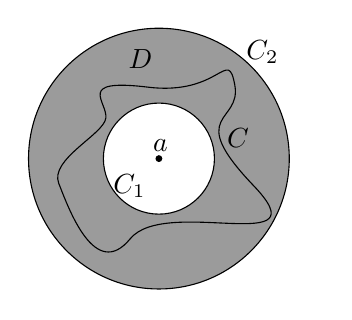
\begin{tikzpicture}[x=0.4,y=0.4,yscale=-1,xscale=1]
%uncomment if require:
\path (0,240.79999542236328);
%set diagram left start at 0, and has height of 240.79999542236328

%Shape: Circle [id:dp6258198346024846] 
\draw  [fill={rgb, 255:red, 155; green, 155; blue, 155 }  ,fill opacity=1 ] (0.77,120.35) .. controls (0.77,55.3) and (53.5,2.57) .. (118.55,2.57) .. controls (183.6,2.57) and (236.32,55.3) .. (236.32,120.35) .. controls (236.32,185.4) and (183.6,238.12) .. (118.55,238.12) .. controls (53.5,238.12) and (0.77,185.4) .. (0.77,120.35) -- cycle ;
%Shape: Circle [id:dp07560041299187703] 
\draw  [fill={rgb, 255:red, 255; green, 255; blue, 255 }  ,fill opacity=1 ] (68.39,120.35) .. controls (68.39,92.65) and (90.85,70.19) .. (118.55,70.19) .. controls (146.25,70.19) and (168.71,92.65) .. (168.71,120.35) .. controls (168.71,148.05) and (146.25,170.51) .. (118.55,170.51) .. controls (90.85,170.51) and (68.39,148.05) .. (68.39,120.35) -- cycle ;
%Shape: Circle [id:dp4185264747557642] 
\draw  [fill={rgb, 255:red, 0; green, 0; blue, 0 }  ,fill opacity=1 ] (116,120.35) .. controls (116,118.94) and (117.14,117.8) .. (118.55,117.8) .. controls (119.96,117.8) and (121.1,118.94) .. (121.1,120.35) .. controls (121.1,121.76) and (119.96,122.9) .. (118.55,122.9) .. controls (117.14,122.9) and (116,121.76) .. (116,120.35) -- cycle ;
%Shape: Polygon Curved [id:ds19792072871438626] 
\draw   (108.6,55.8) .. controls (174.6,63.8) and (180.6,18.8) .. (187.1,53.8) .. controls (193.6,88.8) and (141,78.8) .. (204.1,144.8) .. controls (267.2,210.8) and (124.6,153.8) .. (92.6,192.8) .. controls (60.6,231.8) and (36.72,164.55) .. (28.1,142.8) .. controls (19.47,121.05) and (68.77,98.46) .. (70.6,83.8) .. controls (72.43,69.14) and (42.6,47.8) .. (108.6,55.8) -- cycle ;

% Text Node
\draw (120,108.8) node    {$a$};
% Text Node
\draw (102,30.8) node    {$D$};
% Text Node
\draw (92,144.8) node    {$C_{1}$};
% Text Node
\draw (212,23.8) node    {$C_{2}$};
% Text Node
\draw (190,101.8) node    {$C$};

\end{tikzpicture}

\end{wrapfigure}
複素関数$f(z)$が点$a$を孤立特異点に持つとする。
また、点$a$を中心とする円$C_1, C_2$
($C_1$の中に$a$以外の特異点があっても良く、
$C_2$は$C_1$の外側にあるとする)
によって囲まれる領域を$D$とする。
$C_1, C_2$上、領域$D$のいずれにも特異点がないとき、
領域$D$内の任意の$z$に対し、
$D$内にあって$C_1$を囲むような単純閉曲線$C$を使って
\begin{subequations}
\begin{align}
    f(z)
    &= \sum_{n=-\infty}^{\infty}
        c_n (z-a)^n
\label{Laurent series expansion}
\\
    c_n
    &:= \dfrac{1}{2 \pi i}
    \oint_C dz_0 \dfrac{f(z_0)}{(z_0 - a)^{n+1}}
\end{align}
\end{subequations}
が成り立つ。
これを$f(z)$の$a$周りでのLaurent級数展開という。
特に(\ref{Laurent series expansion})の右辺のうち
$c_{-n}\ (n > 0)$が現れる項を特異部(singular part、主要部、principal part)、
$c_{n}\ (n \ge 0)$が現れる項を正則部(regular part、analytic part)という。

\subsubsection{極(pole)、真性特異点(essential singularity)、零点(zero)}

極とは、以下に定める孤立特異点の一種である。
$f(z)$が$a$を$m\ (>0)$位の極($m$-th order pole)
に持つとは、
$f(z)$のLaurent級数展開が$c_{-m} \neq 0$かつ
$n>m$に対し$c_{-n}=0$を満たすことを言う。
特に$1$位の極を単純極(simple pole)、
$2$位の極を二重極(double pole)、
$3$位ならtriple pole、などともいう。

Laurent展開の特異部が有限次で切れず
負べきの項が無限個現れる場合、
$a$を真性特異点(essential singularity)という。

$f(z)$が$a$を$m$位の零点($m$-th order zero)
に持つとは、
$f(z)$のTaylor級数展開が$c_{m} \neq 0$かつ
$n>m>0$に対し$c_{n}=0$を満たすことを言う。
零点は孤立する。

\subsubsection{留数定理(Residue theorem)}

Laurent級数展開
\begin{align}
    f(z)
    &= \sum_{n=-\infty}^{\infty}
        c_n (z-a)^n
\end{align}
において、
$\Res{f(z)dz, a} := c_{-1}$を
$f(z)$の点$z=a$における留数(Residue)という。
ただし本来これはRiemann球面$\mathbb{C}P^1$上の
微分形式に対し定義されるものだと示すため、
単に$f(z)$ではなく$f(z)dz$と書いた。
特に、
$f(z)$が$a$を$m$位の極
に持つときは
\begin{align}
    \Res{f(z)dz, a}
    =
    \lim_{z \to a}
    \dfrac{1}{(m-1)!}
    \dfrac{d^{m-1}}{dz^{m-1}}
    \bigg[
        (z-a)^m f(z)
    \bigg]
\end{align}
が成り立つ。
$f(z)$が単純閉曲線$C$内で
$n$個の孤立特異点$a_1,\dots,a_n$を除き正則であるとき
\begin{align}
    \oint_C dz\ f(z)
    =
    2 \pi i \sum_{k=1}^n
    \Res{f(z)dz, a_k}
\end{align}
が成り立つ。

\subsubsection{Morera's theorem(モレラの定理)}

以下の意味で、Cauchyの積分定理の逆が成り立つ:
単連結領域$D$で$f(z)$が連続で、
\begin{align}
    \oint_C dz\ f(z) = 0
\end{align}
が$D$内の任意の閉曲線$C$に対し成り立つとする。
このとき$f(z)$は$D$上で正則である。

\subsection{特殊関数}

\subsubsection{指数関数}

指数関数(exponential function)を
\begin{align}
    \exp(x)
    :=
    \sum_{n=0}^\infty
    \dfrac{x^n}{n!}
\end{align}
により定める。
この級数は複素平面全体で絶対収束するため、
$\exp(z)$は整関数
(entire function、複素平面全体で正則な関数)を与える。

\subsubsection{三角関数、双曲線関数}

余弦(cosine)関数、
正弦(sine)関数、
正接(tangent)関数を
指数関数を用いて
\begin{align}
    \cos\theta &:= \dfrac{e^{i\theta} + e^{-i\theta}}{2}
\\
    \sin\theta &:= \dfrac{e^{i\theta} - e^{-i\theta}}{2i}
\\
    \tan\theta &:= \dfrac{\sin\theta}{\cos\theta}
\end{align}
と定義する。
これらを総称して三角関数
(trigonometric function、circular function)
という。

同様に双曲線関数(hyperbolic function)を
\begin{align}
    \cosh\theta
    &:=
    \dfrac{e^{\theta} + e^{-\theta}}{2}
    =
    \cos(-i\theta)
\\
    \sinh\theta
    &:=
    \dfrac{e^{\theta} - e^{-\theta}}{2}
    =
    i\sin(-i\theta)
\\
    \tanh\theta
    &:=
    \dfrac{\sinh\theta}{\cosh\theta}
\end{align}
と定義する。
それぞれ
hyperbolic cosine、
hyperbolic sine、
hyperbolic tangentと言うが、
$\cosh, \sinh, \tanh$の記号は
cosine hyperbolic(またはコッシュ)、
sine hyperbolic(またはシンチ)、
tangent hyperbolic(またはタンチ)
などと発音される。
native English speakerでも
シンチとかタンチとか言う人は居るが、
分かりづらいだけでなく
はっきり言ってクソダサいので
cosine hyperbolic、sine hyperbolic
などという方が良いと思う。

\subsubsection{$\Gamma$関数}

$\Gamma$関数は$\Re z > 0$の複素数$z$に対し
\begin{align}
    \Gamma(z)
    := \int_0^\infty dt\ t^{z-1} e^{-t}
\end{align}
により定義され、
その性質
$\Gamma(1) = 1, \Gamma(z+1) = z\Gamma(z)$
から階乗
\begin{align}
    \Gamma(n+1) &= n!
    \quad
    (n \in \mathbb{N}_{\ge0})
\end{align}
の複素数への一般化を与える。

重要な応用として、
Gaussian integral(ガウス積分)
\begin{align}
    I :=
    \Gamma\left(\dfrac{1}{2}\right)
    =
    \int_{0}^{\infty} dt\ t^{-1/2}e^{-t}
    =
    2
    \int_{0}^{\infty} dx\ e^{-x^2}
    =
    \int_{-\infty}^{\infty} dx\ e^{-x^2}
    > 0
    \quad(t=x^2)
\end{align}
を求める事を考えよう。
極座標に書き換えると
\begin{align}
    I^2 &=
    \int_{-\infty}^{\infty} dx
    \int_{-\infty}^{\infty} dy
    \ 
        e^{-(x^2 + y^2)}
=
    \int_0^{\infty} dr
    \int_0^{2\pi} r d\theta
    \ 
        e^{-r^2}
\notag\\&=
    2 \pi
    \int_0^{\infty} dr
    \ r 
        e^{-r^2}
=
    \pi
    \int_0^{\infty} dt\ e^{-t}
    \quad(t:=r^2,\ dt = 2 r dr)
\notag\\&=
    \pi\Gamma(1)
    = \pi
\end{align}
すなわち
$\Gamma\left(\dfrac{1}{2}\right)
= I = \sqrt{\pi}$
が求まる。

$\Gamma$関数の$\Re z < 0$への解析接続は
Euler's reflection formula
\begin{align}
    \Gamma(z) \Gamma(1-z)
    =
    \dfrac{\pi}{\sin(\pi z)}
\label{Euler's reflection formula}
\end{align}
で与えられ、
この公式からも
$\Gamma \left(\dfrac{1}{2}\right) = \sqrt{\pi}$
が確かめられる。
$\Gamma$関数は零点を持たないが
(\ref{Euler's reflection formula})からも分かるように
$n \in \mathbb{N}_{\ge0}$に対して
$x = - n$を$1$位の極に持ち、
その周りで
\begin{align}
    \Gamma(x)
    &=
    \dfrac{(-1)^n}{n!}
    \left(
        \dfrac{1}{x+n} - \gamma
        + \sum_{k=1}^n \dfrac{1}{k}
    \right)
    + \mathcal{O}(x+n)
\\
    \gamma
    &:=
    \lim_{n\to\infty}
    \left(
        \sum_{k=1}^n \dfrac{1}{k} 
        -
        \log n
    \right)
    \simeq 0.5772
\end{align}
と展開できる。
ただし$\gamma$は
Euler-Mascheroni constant(オイラー定数)である。


\section{量子力学の公式}

\subsection{交換関係・反交換関係の基本的な性質}

証明は読者の演習問題とする。
\begin{align}
    [\hat{A}, \hat{B}] &= - [\hat{B}, \hat{A}]
\\
    [\hat{A}, \hat{B}\hat{C}]
   &=
   \hat{B}[\hat{A}, \hat{C}]
+
    [\hat{A}, \hat{B}] \hat{C}
\label{A,BC to B(A,C) + (A,B)C}
\\
    [\hat{A}\hat{B}, \hat{C}]
   &=
   \hat{A}\{\hat{B}, \hat{C}\}
-
    \{\hat{A}, \hat{C}\} \hat{B}
\\
    \left(\hat{A}\hat{B}\right)^\dagger
    &=
    \hat{B}^\dagger\hat{A}^\dagger
\\
    [\hat{A}, \hat{B}]^\dagger
    &=
    [\hat{B}^\dagger, \hat{A}^\dagger]
\end{align}

Baker-Campbell-Hausdrff formulaは
\begin{align}
    e^{\hat{A}} e^{\hat{B}}
    &=
    \exp\left(
        \hat{A} + \hat{B}
        + \dfrac{1}{2}[\hat{A},\hat{B}]
        + \dfrac{1}{12}[\hat{A} - \hat{B},[\hat{A},\hat{B}]]
        + \cdots
    \right)
\label{BCH formula}
\end{align}
である。証明のためには
$e^{\hat{C}(t)}
= e^{t\hat{A}} e^{t\hat{B}}$
すなわち$\hat{C}(t) = \log (
    e^{t\hat{A}} e^{t\hat{B}}
)$とおき、
右辺のTaylor展開を計算した後
$t=1$とおけばよい。
特に交換関係が$c$-数
$[\hat{A},\hat{B}]=c$の場合は
交換子を$2$回以上取ると必ず消えるため
\begin{align}
    e^{\hat{A}} e^{\hat{A}}
    &=
    \exp\left(
        \hat{A} + \hat{B}
        + \dfrac{1}{2}c
    \right)
\label{simpler BCH formula}    
\end{align}
となる。

正準変数$[\hat{q}_i, \hat{p}_j] = i\hbar\delta_{ij}$
については興味深い事実が成り立つ。
$C_n := \dfrac{1}{i\hbar} [\hat{q}^n_i, \hat{p}_j]$について
\begin{align}
    C_{n+1}
    &=
    \dfrac{1}{i\hbar}
    [\hat{q}^{n+1}_i, \hat{p}_j]
    =
    \hat{q}_i 
    \dfrac{1}{i\hbar}
    [\hat{q}_i^n, \hat{p}_j]
    +
    \dfrac{1}{i\hbar}
    [\hat{q}_i, \hat{p}_j] \hat{q}_i^n
    =
    \hat{q}_i C_n
    +
    \delta_{ij} \hat{q}_i^n
\end{align}
なる漸化式が導けるが、
これは初期条件
$C_0  = 0, C_1 = \delta_{ij}$のもとで
容易に
\begin{align}
    C_{n+1} &= 
    \dfrac{1}{i\hbar}
    [\hat{q}^{n+1}_i, \hat{p}_j]
    = \delta_{ij} (n+1) \hat{q}^n
\label{differential by commutator}
\end{align}
と解け、多項式の微分と同じ振る舞いを与える。
全く同様に
$\dfrac{1}{i\hbar}
[\hat{q}_i, \hat{p}^{n+1}_j]
= \delta_{ij} (n+1) \hat{p}^n$
も示される。
一般にoperatorの関数$F$の定義
(\ref{function of operator})
はTaylor展開で与えられていたので、
\begin{align}
    \dfrac{1}{i\hbar}
    [F(\{ \hat{q} \},\{ \hat{p} \}), \hat{p}_i]
    &=
    \dfrac{
        \partial F(\{ \hat{q} \},\{ \hat{p} \})
    }{
        \partial q_i
    }
\\
    \dfrac{1}{i\hbar}
    [\hat{q}_j, F(\{ \hat{q} \},\{ \hat{p} \})]
    &=
    \dfrac{
        \partial F(\{ \hat{q} \},\{ \hat{p} \})
    }{
        \partial p_j
    }
\end{align}
なる公式が得られる。

任意のoperator $\hat{O}$に対し、
そのHeisenberg表示(Heisenberg描像、Heisenberg picture)を
\begin{align}
    \hat{O}(t)
    :=
    \exp\left(
        -\dfrac{\hat{H} t}{i\hbar}
    \right)
        \hat{O}
    \exp\left(
        +\dfrac{\hat{H} t}{i\hbar}
    \right)
\end{align}
のように定義する。
$\hat{H}$のSchr\"odinger描像とHeisenberg描像は
一致する。
また、もちろんSchr\"odinger描像で
$\hat{O}$自身が顕わに$t$に依存している場合も
Heisenberg描像は同様に定義できる。
Heisenberg描像のoperator
$F(\{ \hat{q} \},\{ \hat{p} \}, t)$と
$\hat{H}$との交換関係は
\begin{align}
    \dfrac{d}{d t}
    F(\{ \hat{q} \},\{ \hat{p} \}, t)
    =
    \dfrac{1}{i\hbar}
    [F(\{ \hat{q} \},\{ \hat{p} \}, t), \hat{H}]
    + \dfrac{\partial}{\partial t}
    F(\{ \hat{q} \},\{ \hat{p} \}, t)
    \label{Heisenberg e.o.m}
\end{align}
となり、Heisenberg equation of motionと呼ばれる。
これはPoisson括弧で書かれた正準方程式(\ref{Hamilton e.o.m. in Poisson bracket})
ないし任意の関数$F$の時間発展(\ref{time evolution in Poisson bracket})
と同一の構造であり、
量子化とは
$\{A, B\}_{ \mathrm{P} }$
を
$\dfrac{1}{i\hbar} [\hat{A}, \hat{B}]$
で置き換える操作である、という
Bohrの対応原理(correspondence principle)をある意味で正当化する。
もちろん\ref{subsubsec: CCR}節で述べたように、
一般にある古典力学系に対して
対応する量子力学系は一意に定まらないので
「古典系を量子化する」という操作はwell-definedではなく、
現代的にはむしろ
量子力学を十分低energyでmacroscopicな系に適用すると
古典力学を再現する、という理解が正しい。


%\begin{align*}
%\end{align*}
%\begin{figure}[!h]
%\centering
%\includegraphics[clip,width=12cm]{}
%\caption{}
%\end{figure}
%\begin{center}
%  \begin{longtable}[H]{|p{5cm}||p{10cm}|}\hline
%\\\hline
%  \end{longtable}
%\end{center}
%\begin{thebibliography}{99}
%\bibitem{primer}
%Stephen P. Martin, A Supersymmetry primer (\href{https://arxiv.org/abs/hep-ph/9709356}{hep-ph/9709356})
%\end{thebibliography}
\end{document}
